\documentclass[11pt]{article}
\usepackage[a4paper, margin=2.54cm]{geometry}
\usepackage[utf8]{inputenc}
\usepackage[spanish, mexico]{babel}
\usepackage[spanish]{layout}
\usepackage{amsmath}
\usepackage{amssymb}
\usepackage{amsfonts}
\usepackage{tikz}
\usepackage{enumerate}
\usetikzlibrary{arrows}

\title{
    Entrega Lógica Borrosa \\
    \large Introducción a la Inteligencia Artificial}
\author{Juan Ignacio Farizano \and Natalia Mellino}
\date{}

\begin{document}
\maketitle
\noindent\rule{\textwidth}{1pt}

\section*{Apartado a)}

\begin{itemize}
\item Variables Linguísticas
  \begin{itemize}
    \item Temperatura $\leftarrow$ variable de entrada
    \item Apertura $\leftarrow$ variable de salida
  \end{itemize}
\item Conjuntos borrosos
  \begin{itemize}
    \item Temperatura fría, temperatura templada, temperatura caliente.
    \item Apertura pequeña, apertura grande.
  \end{itemize}
\end{itemize}

\section*{Apartado b)}

Tenemos que:

\begin{itemize}
    \item El grado de verdad de "la cámara está fría" \ es de 0.7.
    \item El grado de verdad de "la cámara está templada" \ es de 0.3
\end{itemize}

Queremos hallar el grado de verdad de la proposición: "la habitación está fría
o templada". Utilizando la T-conorma con el operador Unión Estándar se tiene que 
el grado de verdad de la proposición viene dado por:
\begin{equation*}
    max(0.7, 0.3) = 0.7
\end{equation*}

Es decir, el grado de verdad de la proposición es 0.7. Al obtenerse un valor
alto, interpretamos este resultado como que la proposición es certera. Lo cual
tiene sentido, ya que como el grado de verdad de "la habitación esta fría" \ es
alto, intuitivamente nos damos cuenta de que probablemente el de la proposición
también lo sea al estar involucrado un "\ o" \ entre habitación fría y habitación
templada. 

\section*{Apartado c)}

\subsection*{Temperatura = 10°}

\begin{itemize}
    \item Se dispararán las reglas 1 y 2 con grado de veracidad 0.5 en ambos casos.
    \item Utilizando la herramienta FisPro con el método de Defuzzificación \emph{mean max}
          se obtiene el siguiente grado de apertura:

          \begin{figure}[h!]
            \begin{center}
              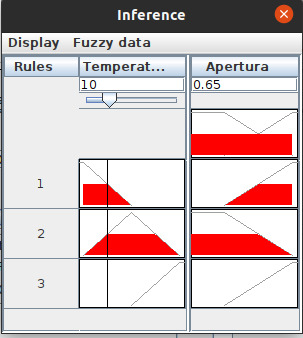
\includegraphics[width=0.4\linewidth]{t10.jpeg}
            \end{center}
          \end{figure}
\end{itemize}

\subsection*{Temperatura = 35°}

\begin{itemize}
    \item Se dispararán las reglas 2 y 3 con grado de veracidad 0.25 y 0.75 respectivamente.
    \item Utilizando la herramienta FisPro con el método de Defuzzificación \emph{mean max}
          se obtiene el siguiente grado de apertura:

          \begin{figure}[h!]
            \begin{center}
              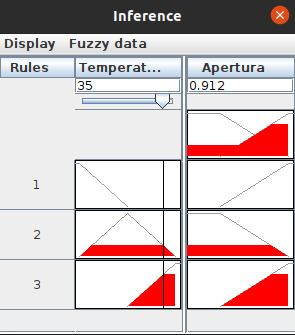
\includegraphics[width=0.4\linewidth]{t35.jpeg}
            \end{center}
          \end{figure}
\end{itemize}

\end{document}